\appendix

\chapter{Nuclear photoeffect and the deuteron}
In this appendix, I wish to go through how to get expressions for the differential cross section and the total cross section from the wave function. The wave function can be obtained analytically or numerically -- in this appendix, I will sketch an analytical approach to $s$-wave calculations. 
Considering the central potential between the proton and the neutron given by
  \[ U(r)= \begin{cases}
        -U_0, & r \leq R \\
        0 & r > R
     \end{cases}
  \]
  The radial equation is given by
  \begin{equation}
  	-\frac{\hbar^2}{2m} \od[2]{u(r)}{r}+\left[U(r)+\frac{\hbar^2 \ell(\ell+1)}{2mr^2} \right]u(r)=Eu(r).
  \end{equation}
\begin{marginfigure}
\centering
\tikzset{every picture/.style={line width=0.75pt}} %set default line width to 0.75pt        

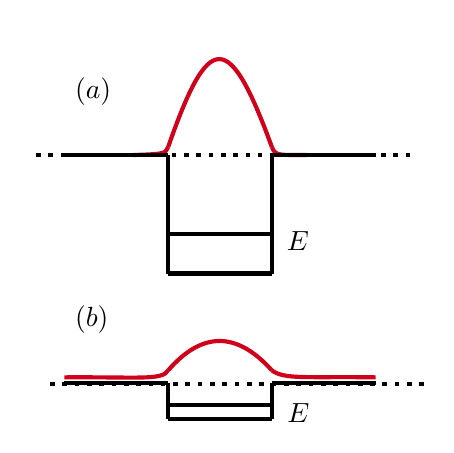
\begin{tikzpicture}[x=0.50pt,y=0.50,yscale=-0.50,xscale=0.50]
%uncomment if require: \path (0,550); %set diagram left start at 0, and has height of 550

%Curve Lines [id:da714237109997598] 
\draw [color={rgb, 255:red, 208; green, 2; blue, 27 }  ,draw opacity=1 ][line width=1.5]    (400,138.65) .. controls (361.29,138.16) and (355.29,140.77) .. (350,127.23) ;
%Curve Lines [id:da6348972322359837] 
\draw [color={rgb, 255:red, 208; green, 2; blue, 27 }  ,draw opacity=1 ][line width=1.5]    (150,138.65) .. controls (198.43,137.18) and (195,136.2) .. (200,127.23) ;
%Straight Lines [id:da38364108936342356] 
\draw [line width=1.5]    (50,138.65) -- (200,138.65) ;
%Straight Lines [id:da9990825563710345] 
\draw [line width=1.5]    (200,138.65) -- (200,310) ;
%Straight Lines [id:da804116660241657] 
\draw [line width=1.5]    (350,138.65) -- (350,310) ;
%Straight Lines [id:da18248652926574438] 
\draw [line width=1.5]    (200,310) -- (350,310) ;
%Straight Lines [id:da7269270295189627] 
\draw [line width=1.5]    (500,138.65) -- (350,138.65) ;
%Straight Lines [id:da9923943428139131] 
\draw [line width=1.5]    (350,252.88) -- (200,252.88) ;
%Curve Lines [id:da9379400250022228] 
\draw [color={rgb, 255:red, 208; green, 2; blue, 27 }  ,draw opacity=1 ][line width=1.5]    (200,127.23) .. controls (259,-42.41) and (288,-42.41) .. (350,127.23) ;
%Straight Lines [id:da2286187239775248] 
\draw [line width=1.5]  [dash pattern={on 1.69pt off 2.76pt}]  (550,138.65) -- (0,138.65) ;
%Curve Lines [id:da32544260892540955] 
\draw [color={rgb, 255:red, 208; green, 2; blue, 27 }  ,draw opacity=1 ][line width=1.5]    (500,460) .. controls (398.33,458.67) and (368.33,463.33) .. (350,450) ;
%Curve Lines [id:da6312090259780904] 
\draw [color={rgb, 255:red, 208; green, 2; blue, 27 }  ,draw opacity=1 ][line width=1.5]    (50,460) .. controls (159,459.25) and (191,464.67) .. (200,450) ;
%Straight Lines [id:da13880877968302263] 
\draw [line width=1.5]    (50,468.65) -- (200,468.65) ;
%Straight Lines [id:da4615629436774523] 
\draw [line width=1.5]    (200,468.65) -- (200,520) ;
%Straight Lines [id:da010903509826977631] 
\draw [line width=1.5]    (350,468.65) -- (350,520) ;
%Straight Lines [id:da9604955519814817] 
\draw [line width=1.5]    (200,500) -- (350,500) ;
%Straight Lines [id:da21767307624229293] 
\draw [line width=1.5]    (500,468.65) -- (350,468.65) ;
%Straight Lines [id:da0797660521308019] 
\draw [line width=1.5]    (350,520) -- (200,520) ;
%Curve Lines [id:da062080896646210415] 
\draw [color={rgb, 255:red, 208; green, 2; blue, 27 }  ,draw opacity=1 ][line width=1.5]    (200,450) .. controls (250,392.27) and (300,394.27) .. (350,450) ;
%Straight Lines [id:da8193626386737687] 
\draw [line width=1.5]  [dash pattern={on 1.69pt off 2.76pt}]  (570,470) -- (20,470) ;

% Text Node
\draw (367,245.28) node [anchor=north west][inner sep=0.75pt]    {$E$};
% Text Node
\draw (61,22.4) node [anchor=north west][inner sep=0.75pt]    {$(a)$};
% Text Node
\draw (368,493.4) node [anchor=north west][inner sep=0.75pt]    {$E$};
% Text Node
\draw (61,352.4) node [anchor=north west][inner sep=0.75pt]    {$(b)$};
\end{tikzpicture}
\caption{Behavior of the ground state bound wave function for two potentials. (a) is an illustration of the deeper potential well case and (b) is for a shallower potential well. }
\end{marginfigure}
  This is identical to the one-dimensional Schrodinger equation with an effective potential, where the centrifugal term pushes the particle outwards. To solve this analytically I rewrite the equation and consider the boundary conditions.
\begin{equation} \label{SEnew}
  \od[2]{u(r)}{r}+\frac{M}{\hbar^2} \left[E-U(r) \right]u(r)=0,
\end{equation}
where I plugged in the expression for the reduced mass, $m=M/2$. For the deuteron I use $E=-E_B = -2.225$ MeV \cite[p. 51]{KerneII}. This leads to the following expressions

\begin{equation} \label{diff1}
  \od[2]{u(r)}{r}+\frac{M}{\hbar^2} \left(U_0-E_B \right)u(r)=0, \quad r \leq R,
\end{equation}
\begin{equation} \label{diff2}
  \od[2]{u(r)}{r}-\frac{M}{\hbar^2} E_B u(r)=0, \quad r > R.
\end{equation}
I introduce two variables given by
\begin{equation} \label{constants}
  k=\sqrt{\frac{M}{\hbar^2}\left(U_0-E_B\right)}, \quad \kappa=\sqrt{\frac{M E_B}{\hbar^2}}.
\end{equation}
Rewriting equation (\ref{diff1}) in terms of (\ref{constants}) and solving the differential equation yields
  \begin{equation} \label{solu1}
  	\od[2]{u(r)}{r} = -ku(r) \Rightarrow u(r) = A\sin(kr)+B\cos(kr).
  \end{equation}
  Since $R(r) = u(r)/r$ and $\cos(kr)/r$ blows up as $r \rightarrow 0 \Rightarrow B=0$ and the solution is
  \begin{equation}
  	u(r)=A\sin(kr), \quad r \leq R
  \end{equation}
  Now, considering equation (\ref{diff2})
  \begin{equation} \label{solu2}
  	\od[2]{u(r)}{r}  = \kappa^2 u(r) \Rightarrow u(r) = Ce^{\kappa r}+De^{-\kappa r}
  \end{equation}
  Here $Ce^{\kappa r}$ blows up as $r\rightarrow \infty$. The wavefunction must be continuous and this means the solutions (\ref{solu1}) and (\ref{solu2}) must match at $r=R$. The same applies for the derivative. This leads to two equations for $r=R$.
  \begin{equation} \label{sin}
  	A\sin(kR) =De^{-\kappa R}
  \end{equation}
  \begin{equation} \label{expo}
  	Ak\cos(kR) =-D\kappa e^{-\kappa R}
  \end{equation}
 \begin{marginfigure}
\centering
\tikzset{every picture/.style={line width=0.75pt}} %set default line width to 0.75pt        

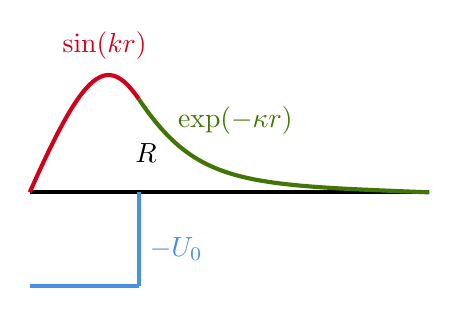
\begin{tikzpicture}[x=0.75pt,y=0.75pt,yscale=-0.90,xscale=0.35]
%uncomment if require: \path (0,891); %set diagram left start at 0, and has height of 891

%Straight Lines [id:da3441756709004927] 
\draw [line width=1.5]    (550,650) -- (0,650) ;
%Straight Lines [id:da3235831888314332] 
\draw [color={rgb, 255:red, 74; green, 144; blue, 226 }  ,draw opacity=1 ][line width=1.5]    (150,650) -- (150,700) ;
%Straight Lines [id:da21114945332143786] 
\draw [color={rgb, 255:red, 74; green, 144; blue, 226 }  ,draw opacity=1 ][line width=1.5]    (150,700) -- (0,700) ;
%Curve Lines [id:da2868941576345746] 
\draw [color={rgb, 255:red, 208; green, 2; blue, 27 }  ,draw opacity=1 ][line width=1.5]    (0,650) .. controls (75,584) and (106,575) .. (150,600) ;
%Curve Lines [id:da577106819832434] 
\draw [color={rgb, 255:red, 65; green, 117; blue, 5 }  ,draw opacity=1 ][line width=1.5]    (150,600) .. controls (230,646) and (293,646) .. (550,650) ;

% Text Node
\draw (41,562.4) node [anchor=north west][inner sep=0.75pt]  [color={rgb, 255:red, 208; green, 2; blue, 27 }  ,opacity=1 ]  {$\varpropto \sin( kr)$};
% Text Node
\draw (200,602.4) node [anchor=north west][inner sep=0.75pt]  [color={rgb, 255:red, 208; green, 2; blue, 27 }  ,opacity=1 ]  {$\textcolor[rgb]{0.25,0.46,0.02}{\varpropto \exp( -\kappa r)}$};
% Text Node
\draw (161,672.4) node [anchor=north west][inner sep=0.75pt]  [color={rgb, 255:red, 208; green, 2; blue, 27 }  ,opacity=1 ]  {$\textcolor[rgb]{0.29,0.56,0.89}{-U_{0}}$};
% Text Node
\draw (141,622.4) node [anchor=north west][inner sep=0.75pt]  [color={rgb, 255:red, 208; green, 2; blue, 27 }  ,opacity=1 ]  {$\textcolor[rgb]{0,0,0}{R}$};


\end{tikzpicture}
\caption{The $s$-wave wave function for the deuteron.}
\end{marginfigure}
  Dividing equation (\ref{expo}) by equation (\ref{sin}) leads to
  \begin{equation} \label{cot}
  	-\cot(kR) = \frac{\kappa}{k}
  \end{equation}
  This equation is solved by requiring $kR=\pi/2$. Plugging in an appropiate value for $R=1.7$ fm yields
  \begin{align*}
  	U_0 & = \frac{\hbar^2\pi^2}{2mR^2}-E \\
  	&= \frac{\hbar^2\pi^2}{2mR^2}+E_B \\
    &= 37.2 \, \text{MeV}
  \end{align*}
This means the depth of the potential is $37.2$ MeV. 

Note that this is all for $s$-wave. Some considerations about the tensor force are also needed. This means we have to consider the Schrödinger equation with noncentral spin-dependent potential given by
\begin{margintable}
\label{Jpi}
\begin{tabular}{lllll}
\toprule
        & $0^+$     & $0^-$   & $1^+$           & $1^-$   \\ \midrule
Singlet & $^{1}s_0$ &         &                 & $^1p_1$ \\
Triplet &           & $3^p_0$ & $^3s_1$,$^3d_1$ & $^3p_1$
\end{tabular}
\caption{Two nucleon states $J^\Pi$. The deuteron consists of a wave function superposition of $^3 s_1+^3d_1$.}
\end{margintable}
\begin{equation}
    \mathcal{U}(r) = \mathcal{U}_0(r) + \mathcal{U}_t(r) S_{12},
\end{equation}
where
\begin{equation}
    \mathcal{U}_t (r) = \mathcal{U}_{tW}(r)+\mathcal{U}_{tM}(r),
\end{equation}
for the space-even states we are considering with the deuteron, see table \ref{Jpi}. Considering the $d$-wave I introduce the anglular momentum coupling $[Y_2(\vec{n})\chi_1]_{1M}$ of spin 1 and $\ell=1$ to the total deuteron spin $J=1$ and projection $J_z = M$. The same coupling but properly normalized can be written as
\begin{equation}
    \Theta_M = \frac{1}{\sqrt{32\pi}} S_{12}\chi_{1M}.
\end{equation}
To get the complete wave function of the deuteron the expression must contain two radial parts and a spherical wave factor $1/r$
\begin{equation}\label{deuteronwave}
    \Psi_M = \frac{1}{\sqrt{4\pi}} \frac{1}{r} \left( u_0(r)+\frac{1}{\sqrt{8}}u_2(r)S_{12}\right)\chi_{1M},
\end{equation}
where the two radial parts are $u_0(r)$ and $u_2(r)$ for $s$-wave and $d$-wave respectivly. These must also be normalized as
\begin{equation}
    \int_0^\infty \textrm{d}r \, \abs{u_0}^2 + \int_0^\infty \textrm{d}r \, \abs{u_2}^2 = 1,
\end{equation}
and the two terms can be interpreted as a weight for the respective wave. Now using the expression for the deuteron wave function equation (\ref{deuteronwave}) I want to get an expression for the differential cross section for the nuclear photoeffect. When an absorbed photon frequency is greater than the lowest threshold of nuclear decay the nucleus becomes excited to the continuum states. These states can decay in a number of ways but here are consider the case where the decay happens through particle emission. In other words this is the absorbtion of a photon that results in a particle decay into the continuum. From conservation of energy we have
\begin{equation}
    E_i = \hbar \omega = E_f + \epsilon,
\end{equation}
where the nucleus $A$ goes from the inital state with energy $E_i$ to the final state with $A-1$ and energy $E_f$ and the particle in the continuum has energy $\epsilon = \vec{p}^2/2m$. 

In contrast to the excitation of the discrete states that shows resonance behavior the continuum of energy states makes for a more smooth dependence. This means we can use what we know form the discrete excitation but introduce a level density $\rho_f$ instead of the usual delta function in the expression for the differential cross section. This yields
\begin{equation}\label{levels}
    \textrm{d}\sigma_{fi} = \frac{4\pi^2\hbar}{E_\gamma c}\abs{\sum_a \frac{\vec{e_a}}{m_a}\mel{f}{(\vec{p}_a\cdot \vec{e}_{\vec{k}\lambda})\textrm{e}^{i(\vec{k}\cdot \vec{r}_a)}}{i}}^2 \rho_f,
\end{equation}
where the level density is given by
\begin{equation}
    \rho_f = \frac{Vmp}{(2\pi\hbar)^3} \textrm{d}o.
\end{equation}
Here the particle is emitted with momentum $\vec{p}$ into the solid angle element $\textrm{d}o$ and $E_\gamma$ is the energy of the photon. In the case of the deuteron equation (\ref{levels}) and be split into different multipolarities and the most simple is the electric dipole transition $(E1)$ from the deuteron bound state into the state of continuum motion of the proton and the neutron with reduced mass $m/2$. 

In the long wave length limit the plane wave expression reduces to unity which means equation (\ref{levels}) for the dipole transition can be written as
\begin{equation} \label{diffE1}
    \textrm{d}\sigma_{E1} = \frac{\alpha mp\omega}{\hbar^2} \abs{\sum_a (\vec{e}\cdot \vec{r_a})_{fi}}^2 \frac{\textrm{d}o}{4\pi},
\end{equation}
where the solid angle could be the direction along the motion of the proton\footnote{Also, $V=1$ and $\alpha=e^2/\hbar c$}.

When assuming an unpolarized deuteron we can take the average over the spin states $1/3 \sum_m$ and count all final polarizations $\sum_{m'}$\footnote{Note $m$ and $m'$}. The final state is still spin triplet since the dipole operator does not act on the spin variable. This yields
\begin{equation} \label{diffcross}
    \overline{\textrm{d}\sigma_{E1}} = \frac{1}{4}\frac{\alpha m p \omega}{\hbar^2} \frac{1}{3} \sum_{mm'}\abs{(\vec{e}\cdot \vec{r})_{fi}}^2 \frac{\textrm{d}o}{4\pi}.
\end{equation}
The task in now to find an expression for the dot product in the sum. The final spin state after the $E1$ transition remains a triplet with $S=J=1$, the orbital and parity, however, is not the same. The final state corresponds to the $p$-wave where the low-energy nuclear forces are weak and the wavelength of the relative motion is much larger than the range of those forces. From conservation of energy we have have
\begin{equation} \label{kq}
    \frac{\hbar^2 k^2}{2m} = \hbar\omega - \epsilon,
\end{equation}
where $\epsilon$ is the binding energy of the deuteron also in equation (\ref{SEnew}). For any direction of the relative momentum vector $\hbar \vec{k}$ the $p$-wave component must be normalized through some Legendre polynomial $P_1(\cos(\theta))$ and the spherical Bessel function $j_{\ell=1}(kr)$.\footnote{$P_1(\cos(\theta))=\cos(\theta)$ and $j_1(\rho)=\frac{\sin(\rho)-\rho\cos(\rho)}{\rho^2}.$}

Here $\theta$ is the angle between the relative coordinate $\vec{r}$ and the wave vector $\vec{k}$ this yields
\begin{equation}
    \psi_f(r,\theta) = 3i\cos(\theta)j_1(kr)\chi_{mm'}
\end{equation}

In the $s$-wave transition we get the following expression when integration over the angles of the unit vector $\vec{n}=\vec{r}/r$
\begin{equation}
    \frac{1}{2}\mel{f;m'}{(\vec{e}\cdot\vec{r})}{\ell=0;m} = -i\frac{\sqrt{\pi}}{k} (\vec{e}\cdot\vec{k} )I_0 \delta_{mm'}.
\end{equation}
The radial integrals for the $s$-wave and $d$-wave are given by $I_0$ and $I_2$ respectively.\footnote{$I_\ell = \int_0^\infty \textrm{d}r \, r^2 j_1(kr)u_\ell(r), \\ \, \, \ell=0,2$}
For the $d$-wave we have to reintroduce the tensor operator\footnote{\begin{align*}
    S_{12}(\vec{n})&=3(\vec{\sigma}_1\cdot \vec{n})(\vec{\sigma}_2)\cdot\vec{n}-(\vec{\sigma}_1\cdot\vec{\sigma}_2) \\
    &= 2[3(\vec{S}\cdot\vec{n})^2-\vec{S}^2]
\end{align*}} $S_12$. Just like in the $s$-wave case we have to integrate over the unit vector -- this time, however, it contains four components
\begin{equation}
    \int \textrm{d}o \, n_i n_j n_k n_l = \frac{4\pi}{15}(\delta{ij}\delta_{kl}+\delta_{ik}\delta_{jl}+\delta_{il}\delta_{jk}),
\end{equation}
and the $d$-wave contribution is given by
\begin{equation}
    \frac{1}{2}\mel{f;m'}{(\vec{e}\cdot \vec{r})}{\ell=2;m} = -i\frac{\sqrt{\pi}}{k}C_{m'm}I_2,
\end{equation}
where the spin matrix element $C_{mm'}$ contains
\begin{equation}\label{operatorC}
    C= \frac{2\sqrt{2}}{5} \Big[ \frac{3}{4}\left[ (\vec{k}\cdot \vec{S})(\vec{e}\cdot \vec{S})+(\vec{e}\cdot \vec{S})(\vec{k}\cdot \vec{S})\right] -(\vec{e}\cdot \vec{k}) \Big].
\end{equation}
Equation (\ref{operatorC}) can be rewritten using a trace identity\footnote{\begin{align*}
    \sum_{mm'}\abs{O_{m'm}}^2=\sum_m (O^\dagger O)_{mm} = \text{Tr}\{ O^\dagger O \}
\end{align*}}
Skipping the calculation and moving back to equation (\ref{diffcross}) we have
\begin{equation}
    \frac{1}{3} \sum_{mm'} \abs{(\vec{e}\cdot \vec{r})_{fi}}^2 = 4\pi \Big(I_0^2\cos^2(\alpha) + \frac{1}{25}I_2^2(3+\cos^2(\alpha)) \Big),
\end{equation}
where $\alpha$ is the angle between $\vec{e}$ and the momentum of the final nucleon $\vec{k}$. The final steps involve averaging over the transverse polarizations of the initial photon which also relates the angle $\alpha$ to the experimentally observed angle between the directions of the photon and final nucleus. This means we get the following expression
\begin{equation} 
    \overline{\cos^2(\alpha)} = \frac{1}{2}\sin^2(\theta)
\end{equation}
Plugging this into equation (\ref{diffE1}) yields
\begin{marginfigure}
\centering
\begin{tikzpicture}[domain=0:pi,scale=1.5]
    \draw[very thick,->] (0,0) -- (pi,0) node[above] {$\theta$};
    \foreach \x in {0, pi/2, pi}
    \draw[thick] (\x, 0.05) -- (\x, -0.05)
        node[anchor=north] {\(\x\)};
    \draw[very thick,->] (0,0) -- (0,2) node[above] {$\textrm{d}\sigma$};
    \draw[color=red, very thick] plot[id=x] function{sin(x)*sin(x)};
\end{tikzpicture}
\caption{Behavior of the differential cross section from equation (\ref{diffcross2}).}
\end{marginfigure}
\begin{equation} \label{diffcross2}
    \textrm{d}\sigma_{E1} = \frac{\pi}{2}\frac{\alpha m p \omega}{\hbar^2} \Big[I_0^2 \sin^2(\theta)+\frac{1}{25}(6+\sin^2(\theta))I_2^2 \Big] \frac{\textrm{d}o}{4\pi},
\end{equation}
and we arrive at the final expression when integrating over the angle of emitted photons
\begin{equation} \label{cross}
    \sigma_{E1} = \frac{\pi}{3}\frac{\alpha m p \omega}{\hbar^2} \Big( I_0^2+\frac{2}{5}I_2^2\Big).
\end{equation}
If is also possible to estimate the cross section in equation (\ref{cross}) using the initial wave function of the approximation of weak binding. Here the wave function is replaced by its exponential tail outside the range of nuclear forces. Furthermore, the contribution $I_2$ is neglected. This means the wave function is given by
\begin{equation}
    \psi_i = \sqrt{\frac{\kappa}{2\pi}} \frac{\textrm{e}^{-\kappa r}}{r},
\end{equation}
where $\kappa$ is defined in equation (\ref{constants}). Calculating the integral $I_0$ yields
\begin{equation}
    \sigma = \frac{8\pi}{3} \frac{\alpha\hbar^2}{M}\frac{\sqrt{\epsilon}(\hbar\omega-\epsilon)^{3/2}}{(\hbar\omega)^3},
\end{equation}
\begin{marginfigure}

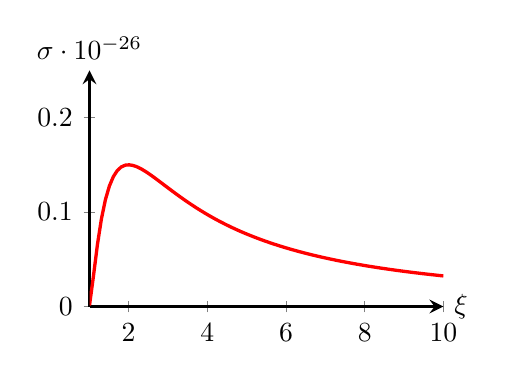
\begin{tikzpicture}

\begin{axis}[
    samples=100,
    domain=0:10, xmax=10, 
    x=0.5cm,
    y=12cm,
    very thick,
    ymin=0, 
    ymax=0.25,
    axis lines=left,
    compat=newest,
    xlabel=$\xi$, xlabel style={at={(1,0)}, anchor=west},
    ylabel=$\sigma\cdot10^{-26}$, ylabel style={rotate=-90,at={(0,1)}, anchor=south}
]
\addplot [red] {1.2*(x-1)^(3/2)*1/(x^3)};
\end{axis}
\end{tikzpicture}
\caption{Behavior of the cross section as a function of photon energy, $\xi$. Maximum occurs at $0.15\cdot10^{-26}$ cm$^2$ which is equivalent to $1.5$ mb. }
\end{marginfigure}

which is rewritten in terms of the photon energy, $\xi = \hbar \omega/\epsilon$ and in terms of numerical estimates
\begin{equation}
    \sigma(\xi) \simeq  1.2\frac{(\xi-1)^{3/2}}{\xi^3}\times 10^{-26} \, \textrm{cm}^2.
\end{equation}